\documentclass{article}

\usepackage{graphicx}
\graphicspath{ {./images/} }

\title{Ch. 22 HW \#2 -- Solutions}
\author{Principles of Microeconomics}
\date{\today}

\begin{document}

\maketitle

\subsection*{Quick Quiz}

\begin{enumerate}

\item (a) -- His budget constraint will rotate inwards.
	
	\begin{center}
	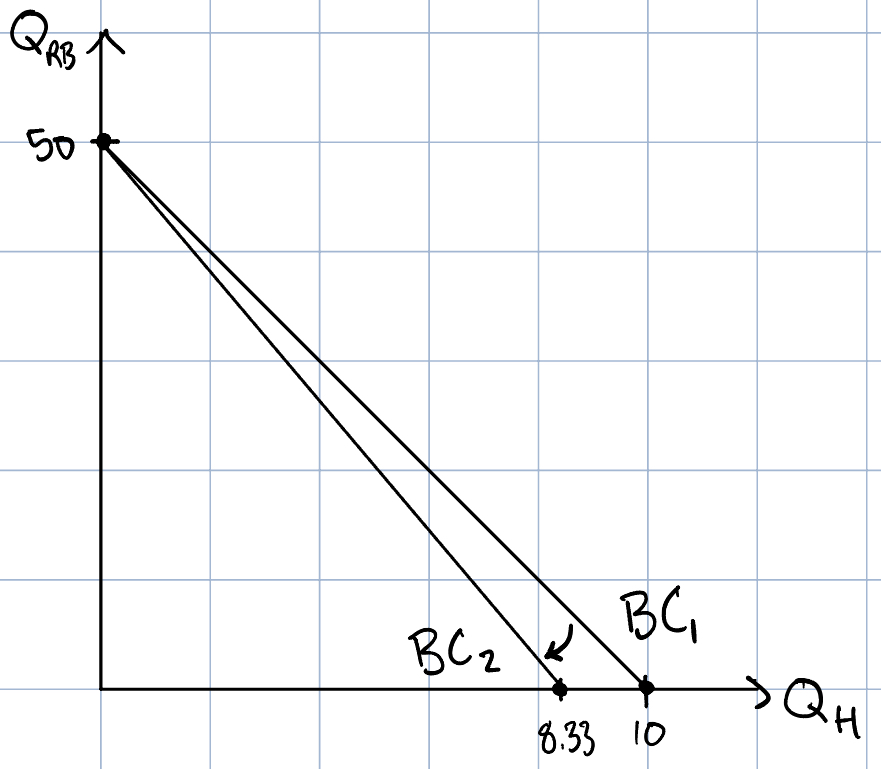
\includegraphics[width = 0.5\textwidth]{qq1}
	\end{center}

\item (d) -- The relative prices remain constant, so the slope of her budget constraint stays the same. Her income rises more than prices rise, so her budget constraint shifts out.

	\begin{center}
	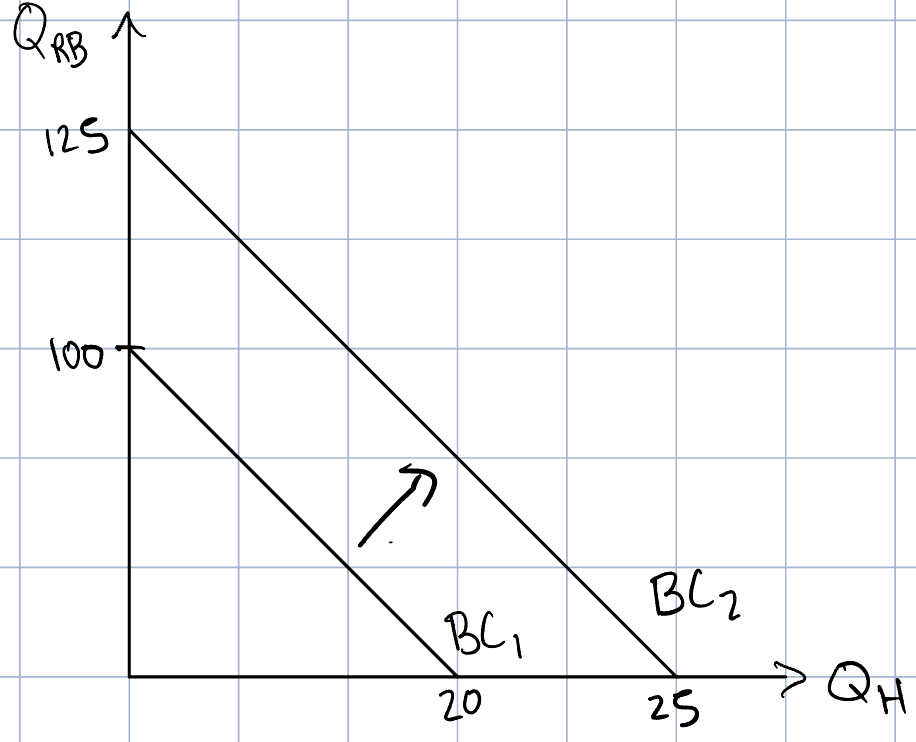
\includegraphics[width = 0.5\textwidth]{qq2}
	\end{center}
	
\item (d) -- A consumer is indifferent between any two points on an indifference curve. In other words, any two consumption bundles on the curve yield the same satisfaction.

\item (b) -- The slope of an indifference curve is the marginal rate of substitution. It's how much of the $y$-axis good the consumer is willing to trade for an additional unit of the $x$-axis good. 

\end{enumerate}

\subsection*{Questions for Review}

\begin{enumerate}

\item The slope is the relative prices of the cheese and wine: $-\frac{P_cheese}{P_wine} = -2$.

	\begin{center}
	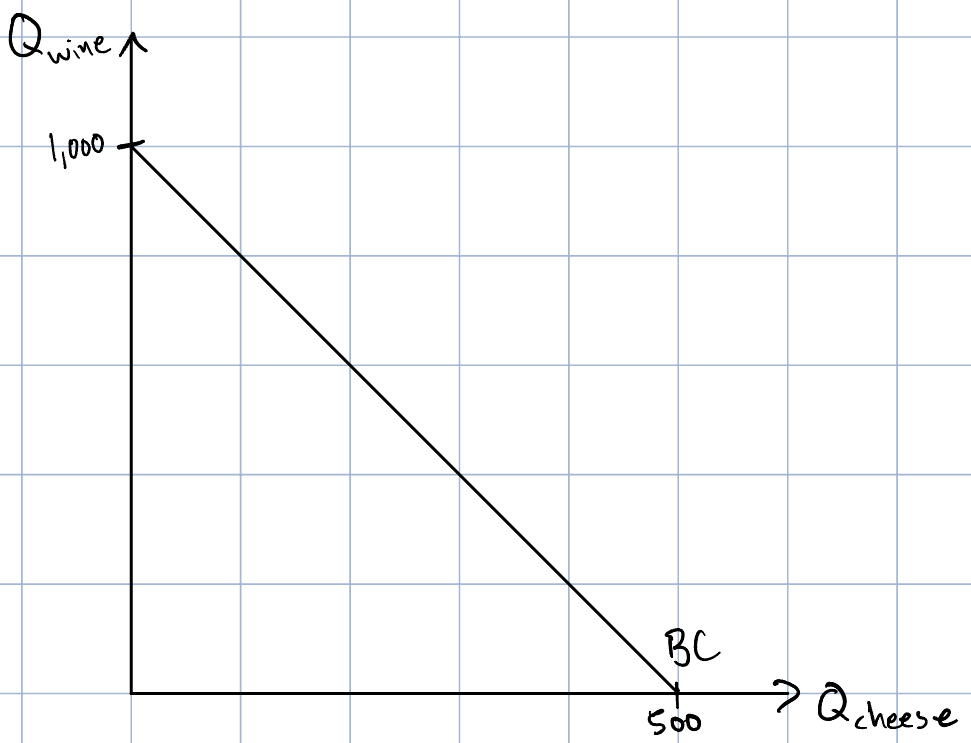
\includegraphics[width = 0.5\textwidth]{qfr1}
	\end{center}
	
\item

	\begin{itemize}
	
	\item Property 1: Higher indifference curves are preferred to lower ones. This is because higher indifference curves include consumption bundles with higher quantities of the goods, and we assume people prefer more consumption over less. 
	
	\item Property 2: Indifference curves slope downwards. If they sloped upwards, the consumer would be indifferent between two bundles where one had more of both goods. That violates our assumption that people prefer more consumption over less.
	
	\item Property 3: Indifference curves don't cross. If they did, it would imply that a consumer was indifferent between two bundles where one had more of both goods. Again, that violates our assumption that people prefer more consumption over less.
	
	\item Property 4: Indifference curves bend towards the origin. We assume that consumers are more willing to give up a good when they have an abundance of it. In other words, the marginal rate of substitution decreases as you move left to right along an indifference curve.
	
	\begin{center}
	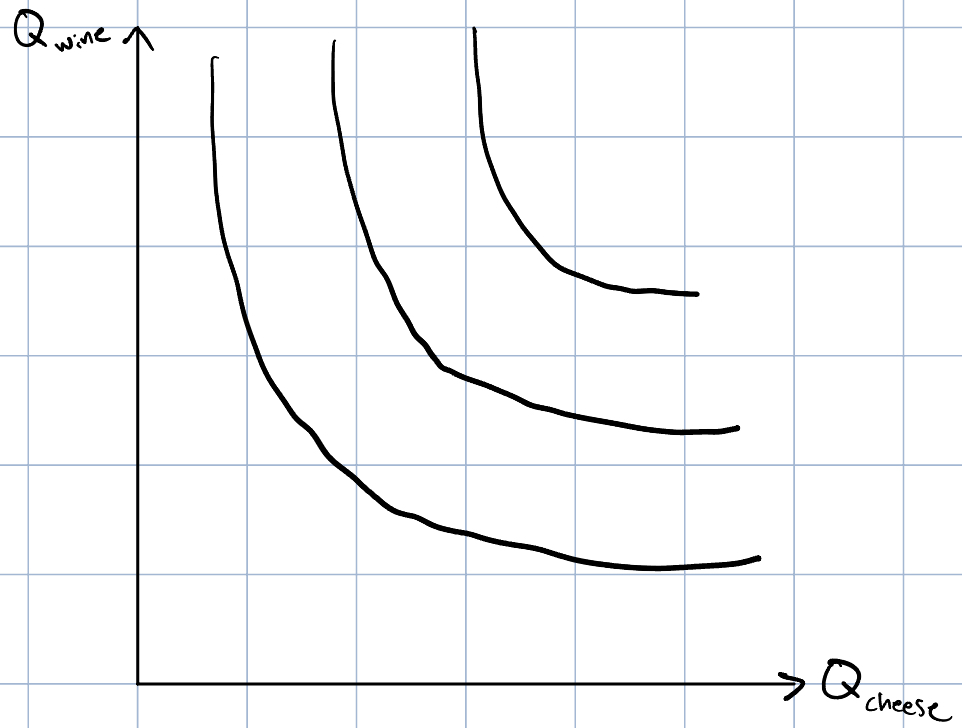
\includegraphics[width = 0.5\textwidth]{qfr2}
	\end{center}
	
	\end{itemize}
	
\item The marginal rate of substitution at $A$ is the slope of the indifference curve at $A$. That's the same thing as the slope of the tangent line at $A$.  Conceptually, it's the quantity of wine the consumer would give up to get another unit of cheese if their current consumption bundle is $A$. 

	\begin{center}
	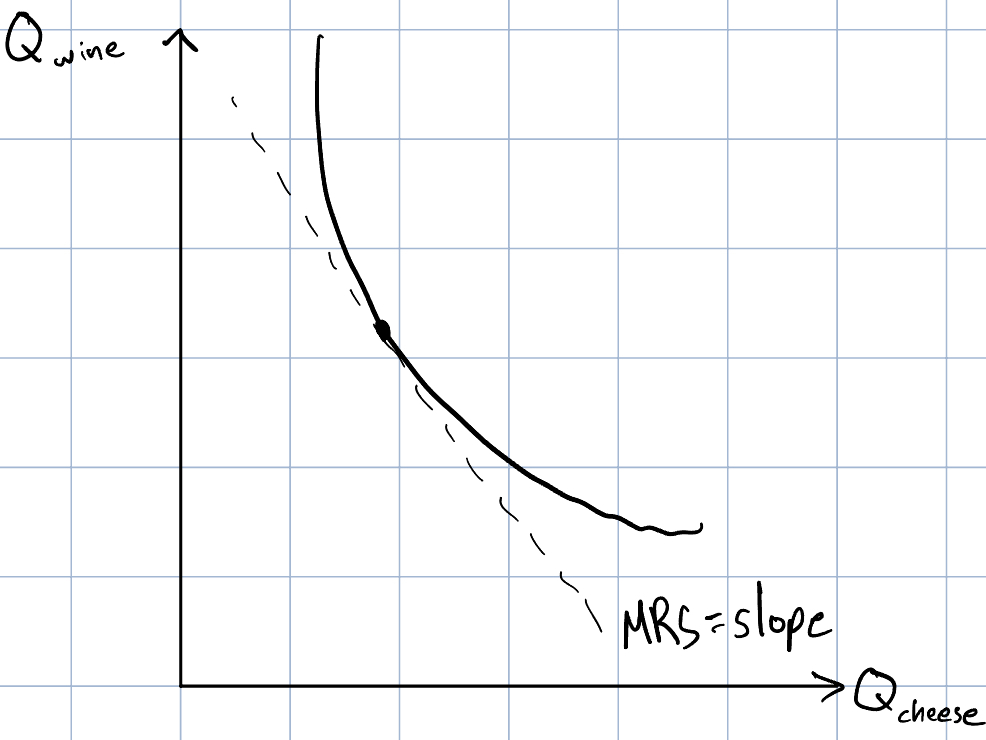
\includegraphics[width = 0.5\textwidth]{qfr3} 
	\end{center}

\end{enumerate}

\end{document}